\section{Performance testing}
To investigate whether or not the primitives provided were suitable for the task we implemented three benchmarks designed to be as similar as possible to real world scenarios.


\subsection{Devices}
Different devices were employed for testing. Table \ref{table:devices-used} provides a correspondence between names used in the graphs and the mark and model of the devices 
used.

\begin{table}[h]
\centering
\caption{Devices used for performance testing}
\label{table:devices-used}
\begin{tabular}{lllll}
\hline
Name          & Manufacturer      & Model name    \\ \hline
Nexus 5       & Google            & Nexus 5       \\
Nexus 7       & Google            & Nexus 7       \\
OnePlus One 1 & OnePlus           & One           \\
OnePlus One 2 & OnePlus           & One           \\
Redmi         & Xiaomi            & Redmi 2       \\ 
\hline
\end{tabular}
\end{table}

\subsection{Throughput}
This benchmark was designed to test the transmission performance of Bluetooth in the context of a long lasting connection to a single other device such as the exchange of a picture or video.
Transmission performance is defined in terms of bytes transferred per second.

A single run of the test involved two devices: a server which sent packets of a predefined size and a client which received the packets and computed the time necessary to receive them.
The test was then run between each pair of devices and the results are shown in Figure \ref{figure:throughput}.

\begin{figure}[ht!]
  \centering
  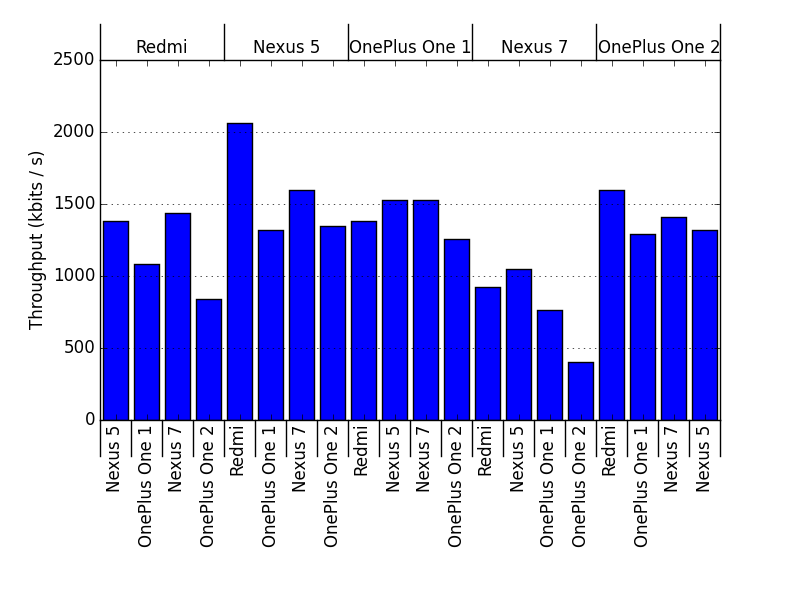
\includegraphics[width=1.0\textwidth]{img/throughput.png} 
  \caption{KBytes received per second. Devices on the top are servers while devices on the bottom are clients.}
  \label{figure:throughput}
\end{figure}

\subsection{Round trip time}
In an application designed to allow people to communicate, the time a message takes to be delivered is an important parameter.
The delivery time can be split into two parts, the setup of the connection and the delivery itself.
Understanding how much time is spent on each of this two phases is critical in designing an efficient protocol.

The benchmark tested the connection setup cost and round trip time of messages of various sizes.
In order to make sure that the network wasn't loaded and the connection setup cost was being evaluated correctly only one device at a time could send messages.
The protocol works as follows:

\begin{enumerate}
\item At the beginning of the test a random device is assigned a token
\item The device holding the token selects another peer to communicate with
\item A message is sent to the other peer which answers with a reply message
\item The connection setup cost and round trip time are computed
\item The token is passed to the other device
\item Steps 2 to 5 are repeated a configurable amount of times
\end{enumerate}

The data collected is show in \ref{figure:rtt}.

\begin{figure}[ht!]
  \centering
  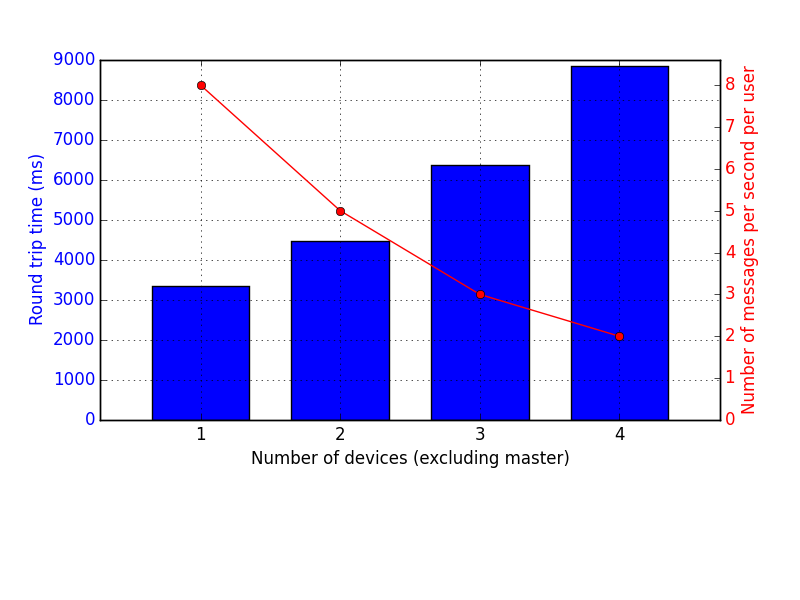
\includegraphics[width=1.0\textwidth]{img/messages_per_second.png} 
  \caption{Estimate of Round Trip Time and Messages per second rate}
  \label{figure:messages-per-second}
\end{figure}